\hyperdef{}{tilda}{}

\subsection{\texorpdfstring{{Variablen}}{Variablen}}

\subsubsection{\texorpdfstring{{\ldots{} im
Allgemeinen}}{\ldots{} im Allgemeinen}}

\par\noindent\textbf{Was ist eine Variable?}

\begin{itemize}
\itemsep1pt\parskip0pt\parsep0pt
\item
  {\emph{Variable} ist das Substantiv zu \emph{variabel}, welches auf
  Latein \emph{variabilis} ``veränderbar'' zurückgeht.}
\item
  {Eine Variable ist also etwas, das änderbar ist.}
\item
  {Johnny Depp ist ein Beispiel für eine \emph{Variable}, weil er sehr
  änderbar ist, wie man an seinen Filmen sehen kann.}
\end{itemize}



\par\noindent\textbf{\href{http://de.wikipedia.org/wiki/variable_(programming)}{Wikipedias
Definition}:}

\begin{quote}
In computer programming, a variable is a symbolic name given to some
known or unknown quantity or information, for the purpose of allowing
the name to be used independently of the information it represents. A
variable name in computer source code is usually associated with a data
storage location and thus also its contents, and these may change during
the course of program execution.
\end{quote}



\par\noindent\textbf{Definition in
\href{http://bibliography.lingpy.org?key=Puttkamer1990}{Puttkamer
(1990)}:}

\begin{quote}
Bei jeder Art von Datenverarbeitung beziehen sich die Anweisungen auf
direkte Daten, die eingegeben werden oder auf Variable, die man sich
vorstellen kann als mit Namen versehen Behälter für Daten. Jede
Zuweisung an eine Variable füllt Daten in diesen Behälter, und der Wert
einer Variablen ist der Inhalt dieses Behälters. So ist z. B. der Effekt
einer Anweisung \$A:= 3 + 7\$: Bilde mit den direkt eingegebenen Daten 3
und 7 die Summe 10 und weise diesen Wert der Variablen mit Namen A zu.
Ein {[}sic!{]} anschließende Anweisung ``drucke A'' druckt den Inhalt
des Behälters A aus, den Wert der Variablen A, hier 10.
\end{quote}



\par\noindent\textbf{Vereinfachte Begriffserklärung}

\begin{itemize}
\itemsep1pt\parskip0pt\parsep0pt
\item
  {Beim Programmieren werden Werte benötigt, deren Inhalt variabel ist.}
\item
  {Variabel heißt, dass die Werte sich entweder bei jedem erneuten
  Programmaufruf ändern können, oder sogar innerhalb des Programms.}
\item
  {Bspw. lässt sich ein Programm, dass eine Ganzzahl mit sich selbst
  multipliziert und das Ergebnis dieser Multiplikation wieder mit sich
  selbst, nicht schreiben, wenn man nicht eine Möglichkeit hat, auf die
  Zahl zuzugreifen, obwohl man sie noch nicht kennt.}
\item
  {Variablen ermöglichen derartige Programmoperationen.}
\item
  {Variablen sind Platzhalter, die, wenn das Programm ausgeführt wird,
  mit einem Wert gefüllt werden (\emph{Deklaration}).}
\end{itemize}


\subsubsection{\texorpdfstring{{\ldots{} in
Python}}{\ldots{} in Python}}

\par\noindent\textbf{Deklaration von Variablen in Python}

\begin{verbatim}
>>> VARIABLE = VALUE
>>> VAR1, VAR2, ... = VAL1, VAL2, ...
>>> VAR1, \*VAR2 = VAL1, VAL2, VAL3, ...
>>> VARIABLE = VAL1, VAL2, ...
\end{verbatim}

\begin{verbatim}
>>> a = 1
>>> b, c = 2, 3
>>> d, \*e = 4, 5, 6
>>> f = 7, 8, 9
>>> print(myvar, myvar1, myvar2, myvar3, myvar4, myvar5)
1 2 3 4 [5, 6] (7, 8, 9)
\end{verbatim}



\par\noindent\textbf{Struktur von Variablennamen}

\begin{verbatim}
>>> Name = 1
>>> Name_von_mir = 1
>>> Name2 = 1
\end{verbatim}

\begin{verbatim}
>>> 2Name = 1
SyntaxError: invalid syntax
\end{verbatim}



\par\noindent\textbf{Programmierbeispiele}

\begin{verbatim}
>>> print("Variable")
Variable
>>> Variable = "Variable"
>>> print(Variable)
Variable
>>> Variable
'Variable'
>>> Variable == Variable
True
Variable == 'Variable'
True
>>> var1, var2 = 2, 3
>>> print(var1,"und", var2,"macht",var1 + var2)
2 und 3 macht 5
\end{verbatim}



\par\noindent\textbf{Fehlermeldungen}

\begin{verbatim}
>>> test = 1,2
>>> test = bla
Traceback (most recent call last):
  File "<stdin>", line 1, in <module>
NameError: name 'bla' is not defined
\end{verbatim}

\begin{verbatim}
>>> print(test1)
traceback (most recent call last):
  file "<stdin>", line 1, in <module>
nameerror: name 'test1' is not defined
\end{verbatim}

\begin{verbatim}
>>> test1 = 2
>>> test2 = "2"
>>> test1 + test2
Traceback (most recent call last):
  File "<stdin>", line 1, in <module>
TypeError: unsupported operand type(s) for +: 'int' and 'str'
\end{verbatim}


\subsubsection{\texorpdfstring{{\ldots{} in
JavaScript}}{\ldots{} in JavaScript}}

\par\noindent\textbf{Deklaration von Variablen in JavaScript}

\begin{verbatim}
> VARIABLE = 1;
> var VAR = 1;
> VAR1 = 1; VAR2 = 2;
> var VAR1, VAR2;
> VAR1 = 1; VAR2 = 1;
\end{verbatim}

{Das Schlüsselwort ``var'' wird in JavaScript verwendet, um
sicherzustellen, dass Variablen in Funktionen lokal definiert werden.
Grundsätzlich sollte man (da wir ohnehin nicht global definieren
sollten) darauf achten, immer das Schlüsselwort ``var'' einer
Variablendeklaration vorwegzustellen.}



\par\noindent\textbf{Struktur von Variablennamen}

\begin{verbatim}
> var Name = 1
> var Name_von_mir = 1
> var Name2 = 1
\end{verbatim}

\begin{verbatim}
> var 2Name = 1
SyntaxError: identifier starts immediately after numeric literal
\end{verbatim}



\par\noindent\textbf{Programmierbeispiele}

\begin{verbatim}
> var myvar = 1;
> var myvar2 = 2;
> var myvar3, myvar4, myvar5;
> myvar3 = 3; myvar4 = 4; myvar5 = 5;
> [myvar1, myvar2, myvar3, myvar4, myvar5].map(function(x){return x+x});
[ 2, 4, 6, 8, 10 ]
\end{verbatim}



\par\noindent\textbf{Fehlermeldungen}

\begin{verbatim}
> var a = 10;
> var b = '11';
> a + a;
20
> b + b;
1111
> a + b
1011
> a - "10";
0
> a * "10";
100
\end{verbatim}

{Vorsicht mit den Operatoren +, -, * und / in JavaScript! Ihr Verhalten
kann unberechenbar sein, da im Gegensatz zu Python kein Typcheck
durchgeführt wird!}

\subsection{\texorpdfstring{{Datentypen}}{Datentypen}}

\subsubsection{\texorpdfstring{{\ldots{} im
Allgemeinen}}{\ldots{} im Allgemeinen}}

\par\noindent\textbf{\href{http://de.wikipedia.org/wiki/Datentyp}{Wikipedia-Definition:}}

\begin{quote}
Formal bezeichnet ein Datentyp in der Informatik die Zusammenfassung von
Objektmengen mit den darauf definierten Operationen. Dabei werden durch
den Datentyp des Datensatzes unter Verwendung einer so genannten
Signatur ausschließlich die Namen dieser Objekt- und Operationsmengen
spezifiziert. Ein so spezifizierter Datentyp besitzt noch keine
Semantik. Die weitaus häufiger verwendete, aber speziellere Bedeutung
des Begriffs Datentyp stammt aus dem Umfeld der Programmiersprachen und
bezeichnet die Zusammenfassung konkreter Wertebereiche und darauf
definierten Operationen zu einer Einheit. Zur Unterscheidung wird für
diese Datentypen in der Literatur auch der Begriff Konkreter Datentyp
verwendet. Für eine Diskussion, wie Programmiersprachen mit Datentypen
umgehen, siehe Typisierung.
\end{quote}



\par\noindent\textbf{Vereinfachte Begriffserklärung}

\begin{itemize}
\itemsep1pt\parskip0pt\parsep0pt
\item
  {Variable als Platzhalter, der mit einem bestimmten Wert gefüllt
  wird.}
\item
  {Worum es sich bei dem Wert handelt, ist wichtig für die korrekte
  Durchführung eines Programms.}
\item
  {Wörter kann man beispielsweise nicht addieren.}
\item
  {Zahlen kann man dafür nicht einfach aneinanderreihen.}
\item
  {Auch im wirklichen Leben teilen wir unsere Zeichen in gewisser Weise
  in Datentypen ein, denn wenn wir den Satz ``Multipliziere mal 1 und
  1'' hören, dann denken wir bei ``1'' an eine Zahl und nicht an eine
  Zeugnisnote, weil man eine Zeugnisnote nicht multiplizieren kann.}
\end{itemize}


\subsubsection{\texorpdfstring{{\ldots{} in
Python}}{\ldots{} in Python}}

\par\noindent\textbf{Allgemeines}

In Python werden Datentypen bei der Variablendeklaration nicht explizit
angegeben, sondern aufgrund der Struktur der Werte, die den Variablen
zugewiesen werden, automatisch bestimmt. Python weist eine Vielzahl von
Datentypen auf und ermöglicht aufgrund seiner objektorientierten
Ausrichtung auch die Erstellung eigener komplexer Datentypen.



\par\noindent\textbf{Wichtigste Datentypen in Python}

\begin{itemize}
\itemsep1pt\parskip0pt\parsep0pt
\item
  {\emph{integer}: fasst ganzzahlige Werte (\texttt{2,\ 3,\ -5,\ 0})}
\item
  {\emph{float}: fasst Fließkommawerte
  (\texttt{1.2,\ 1.222,\ -0.5,\ -2.5})}
\item
  {\emph{string}: fasst Zeichenketten
  (\texttt{"Friedrich",\ "Nietzsche",\ "孔子"})}
\item
  {\emph{list}: fasst jede Art von anderen Datentypen in linearer
  Anordung und kann verändert werden
  (\texttt{{[}"Friedrich",\ "2",\ 1998,\ -0.5{]}})}
\item
  {\emph{tuple}: fasst jede Art von anderen Datentypen, kann aber nicht
  verändert werden ( \texttt{("Friedrich",\ "2",\ 1998,\ -0.5)})}
\item
  {\emph{dict}: fasst jede Art von anderen Datentypen als Sammlung von
  Key-Value-Paaren, vobei der Key weder Liste noch Dictionary sein kann
  (\texttt{\{1:1,\ "Friedrich"\ :\ "Nietzsche"\}})}
\end{itemize}



\par\noindent\textbf{Überprüfen}

\begin{verbatim}
>>> a, b, c, d = 1, "2", 2.5, [1,2]
>>> type(a)
<class 'int'>
>>> print(type(b), type(c))
<class 'int'> <class 'str'>
>>> isinstance(d, list)
True
>>> isinstance(d, (int,str))
False
\end{verbatim}


\par\noindent\textbf{Programmbeispiele}

\begin{verbatim}
>>> a, b, c = 1, "2", 3.5
>>> words = ["apfel", "wurst", "gurke"]
>>> nahrungs_typ = {"apfel": "vegan", "wurst": "carnivor", "gurke": "vegan"}
>>> b + b
'22'
>>> a / c
-2.5
>>> type(a/c)
<class 'float'>
>>> for word in words: print(word, nahrungs_typ[word])
apfel vegan
wurst carnivor
gurke vegan
>>> print(words[1])
wurst
\end{verbatim}


\subsubsection{\texorpdfstring{{\ldots{} in
JavaScript}}{\ldots{} in JavaScript}}

\par\noindent\textbf{Allgemeines}

Auch in JavaScript werden Datentypen bei der Deklaration nicht explizit
angegeben, sondern dynamisch bestimmt. Auch in JavaScript können
komplexe Datentypen aufgrund der Möglicheit, objekt-orientiert zu
programmieren, erstellt werden. Im Gegensatz zu Python ist es viel
leichter, Operationen auf unterschiedlichen Datentypen durchzuführen,
was problematisch werden kann, da die erwarteten Ergebnisse sich leicht
unterscheiden können, wenn ein Programm nicht sorgfälgit geprüft wird.



\par\noindent\textbf{Wichtigste Datentypen in Javascript}

\begin{itemize}
\itemsep1pt\parskip0pt\parsep0pt
\item
  {\emph{number}: Ganz- und Fließkommazahlen (\texttt{1,\ 1.5})}
\item
  {\emph{string}: Zeichenketten
  (\texttt{"hallo",\ \textquotesingle{}welt\textquotesingle{}})}
\item
  {\emph{array}: linear angeordnete variable Datentypen
  (\texttt{{[}1,\ "2",\ -3{]}})}
\item
  {\emph{object}: Key-Value-Paare (\texttt{\{0:1,\ 1:2\}})}
\end{itemize}

{Beachten Sie, dass es sich bei dem Datentyp ``array'' offiziell um eine
spezielle Form des sehr abstrakten Datentypen ``object'' handelt,
weshalb ein Type-Check auch für einen Array immer den Wert ``object''
zurückliefern wird.}



\par\noindent\textbf{Überprüfen}

\begin{verbatim}
> var a = 1;
> var b = 1.5;
> var c = "1";
> var d = [a, b, c];
> var e = {0 : a, 1 : b, 2 : c};
> typeof a;
number
> typeof b;
number
> typeof c;
string
> typeof d;
object
> typeof e;
object
\end{verbatim}



\par\noindent\textbf{Programmbeispiele}

\begin{verbatim}
> var a = 1;
> var b = 1.5;
> var c = "1";
> var d = [a, b, c];
> var e = {0 : a, 1 : b, 2 : c};
> a == d[0];
True
> a === d[0];
True
> e[0] = 2
for (key in e) {alert(key+' '+e[key])}
\end{verbatim}

\subsection{\texorpdfstring{{Praktische
Beispiele}}{Praktische Beispiele}}

\subsubsection{\texorpdfstring{{Die
Dreiballkaskade}}{Die Dreiballkaskade}}

\par\noindent\textbf{\href{http://de.wikipedia.org/wiki/Kaskade_(Jonglieren)}{Dreiballkaskade
in Wikipedia}}

\begin{quote}
Als Kaskade wird das am einfachsten zu erlernende Jongliermuster mit
einer ungeraden Anzahl von Gegenständen (Zum Beispiel: Bällen, Keulen
oder Ringen) bezeichnet. Dabei wird mit zwei Gegenständen in einer Hand
und einem in der anderen Hand angefangen. Der erste Wurf wird durch die
Hand ausgeführt, in der zwei Gegenstände sind. Wenn der Gegenstand den
höchsten Punkt erreicht, wird der Gegenstand aus der anderen Hand
losgeworfen (und zwar unter dem zuvor geworfenen Gegenstand hindurch).
Dadurch ist diese Hand frei, um den ersten Gegenstand zu fangen. Wenn
der zweite Gegenstand am höchsten Punkt angekommen ist, wird der dritte
Gegenstand losgeworfen (mit der Hand, die auch den ersten Gegenstand
geworfen hat) und so weiter.
\end{quote}



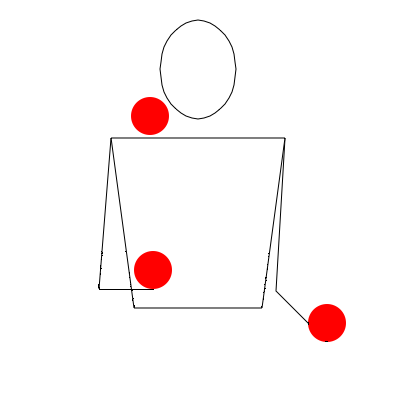
\includegraphics{img/3-ball_cascade_movie.png}


\subsubsection{\texorpdfstring{{Die Dreiballkaskade in
Python}}{Die Dreiballkaskade in Python}}

\begin{verbatim}
# definiere das jongliermuster
JonglierMuster = """
\n\n\n\n\n\n\n\n\n\n\n\n\n\n\n\n\n\n\n\n\n\n\n\n\n\n\n\n\n\n\n\n\n\n\n\n\n\n
  Dreiball-Jonglage      
+-------------------+
| (L)           (R) |
|                   |
|                   |
|                   |
|                   |
||(l)|         |(r)||
|  |             |  |               
+-------------------+
"""

# deklariere die gegenstände
gegenstand1 = '(1)'
gegenstand2 = '(2)'
gegenstand3 = '(3)'

# halte fest, welcher gegenstand gerade wo ist
RechteHand = gegenstand2
LinkeHand = gegenstand3
RechtsOben = gegenstand1
LinksOben = '   '

# Jetzt kann es losgehen. Das Programm startet, indem wir die Entertaste
# drücken.
input("Los geht's!")

# Wir führen eine Schleife aus (Details dazu kommen später)
i = 0
while i < 20:

    # wir deklarieren eine variable snapshot, die in jeweils vier schritten
    # durch das derzeit vorliegende jongliermuster ersetzt wird
    SnapShot = JonglierMuster
    SnapShot = SnapShot.replace('(R)',RechtsOben)
    SnapShot = SnapShot.replace('(L)',LinksOben)
    SnapShot = SnapShot.replace('(l)',LinkeHand)
    SnapShot = SnapShot.replace('(r)',RechteHand)

    # Wir benutzen nicht print, um das ganze auszugeben, sondern input(),
    # weil damit immer gleichzeitig auch eine Pause verbunden ist (erst wenn
    # man Enter drückt geht es weiter). (in Python2 brauchen wir "raw_input")
    input(SnapShot)

    # jetzt passen wir die variablen an, wobei wir schauen, wo gerade der
    # ball ist.
    if RechtsOben == '   ':
        RechtsOben = LinkeHand
        LinkeHand = '   '
        i += 1

    elif RechteHand == '   ':
        RechteHand = RechtsOben
        RechtsOben = '   '
        i += 1

    elif LinkeHand == '   ':
        LinkeHand = LinksOben
        LinksOben = '   '
        i += 1

    elif LinksOben == '   ':
        LinksOben = RechteHand
        RechteHand = '   '
        i += 1

# Wenn alles geschafft ist, kann man schon mal darauf hinweisen, dass das
# ziemlich anstrengend ist...
input("Puh, war das anstrengend!")
\end{verbatim}



Dies ist eine Python-2 Version, das heißt, dass die Funktion ``input''
durch ``raw\_input'' ersetzt werden muss:


\subsubsection{\texorpdfstring{{Die Dreiballkaskade in
Javascript}}{Die Dreiballkaskade in Javascript}}

\par\noindent\textbf{HTML Kode}

\begin{verbatim}
<html>
<head>
  Kaskade Demo
  
</head>

  
    
      
      
      
      (1)
    
           
    
      (2)
      
      
      (3)
    
  
  Next Catch
  ...
\end{verbatim}



\par\noindent\textbf{CSS Kode}

\begin{verbatim}
.white {
  color: red;
  width: 50px;
  height: 50px;
  background: lightgray;
}
.hand {
  border-bottom: 10px solid Orange;
}
.right {
  border-right: 10px solid Orange;
}
.left {
  border-left: 10px solid Orange;
}

.ball {
  font-size: 20px;
  color: Crimson;
  font-weight: bold;
  text-align: center;
  background: lightgray;
}
\end{verbatim}



\par\noindent\textbf{JavaScript Kode}

\begin{verbatim}
function nextCatch() {

  // get items for all the values in the cells
  var ro = document.getElementById('ro');
  var lo = document.getElementById('lo');
  var ru = document.getElementById('ru');
  var lu = document.getElementById('lu');

  console.log(ro.innerHTML, lo.innerHTML);

  // get emtpy value 
  if (ro.innerHTML == '') {
    ro.innerHTML = lu.innerHTML;
    lu.innerHTML = '';
  }
  else if (lo.innerHTML == '') {
    lo.innerHTML = ru.innerHTML;
    ru.innerHTML = '';
  }
  else if (lu.innerHTML == '') {
    lu.innerHTML = lo.innerHTML;
    lo.innerHTML = '';
  }
  else if (ru.innerHTML == '') {
    ru.innerHTML = ro.innerHTML;
    ro.innerHTML = '';
  }
}
\end{verbatim}

\par\noindent\textbf{DEMO}

